% Options for packages loaded elsewhere
\PassOptionsToPackage{unicode}{hyperref}
\PassOptionsToPackage{hyphens}{url}
\PassOptionsToPackage{dvipsnames,svgnames,x11names}{xcolor}
%
\documentclass[
  letterpaper,
  DIV=11,
  numbers=noendperiod]{scrartcl}

\usepackage{amsmath,amssymb}
\usepackage{iftex}
\ifPDFTeX
  \usepackage[T1]{fontenc}
  \usepackage[utf8]{inputenc}
  \usepackage{textcomp} % provide euro and other symbols
\else % if luatex or xetex
  \usepackage{unicode-math}
  \defaultfontfeatures{Scale=MatchLowercase}
  \defaultfontfeatures[\rmfamily]{Ligatures=TeX,Scale=1}
\fi
\usepackage{lmodern}
\ifPDFTeX\else  
    % xetex/luatex font selection
\fi
% Use upquote if available, for straight quotes in verbatim environments
\IfFileExists{upquote.sty}{\usepackage{upquote}}{}
\IfFileExists{microtype.sty}{% use microtype if available
  \usepackage[]{microtype}
  \UseMicrotypeSet[protrusion]{basicmath} % disable protrusion for tt fonts
}{}
\makeatletter
\@ifundefined{KOMAClassName}{% if non-KOMA class
  \IfFileExists{parskip.sty}{%
    \usepackage{parskip}
  }{% else
    \setlength{\parindent}{0pt}
    \setlength{\parskip}{6pt plus 2pt minus 1pt}}
}{% if KOMA class
  \KOMAoptions{parskip=half}}
\makeatother
\usepackage{xcolor}
\setlength{\emergencystretch}{3em} % prevent overfull lines
\setcounter{secnumdepth}{5}
% Make \paragraph and \subparagraph free-standing
\ifx\paragraph\undefined\else
  \let\oldparagraph\paragraph
  \renewcommand{\paragraph}[1]{\oldparagraph{#1}\mbox{}}
\fi
\ifx\subparagraph\undefined\else
  \let\oldsubparagraph\subparagraph
  \renewcommand{\subparagraph}[1]{\oldsubparagraph{#1}\mbox{}}
\fi


\providecommand{\tightlist}{%
  \setlength{\itemsep}{0pt}\setlength{\parskip}{0pt}}\usepackage{longtable,booktabs,array}
\usepackage{calc} % for calculating minipage widths
% Correct order of tables after \paragraph or \subparagraph
\usepackage{etoolbox}
\makeatletter
\patchcmd\longtable{\par}{\if@noskipsec\mbox{}\fi\par}{}{}
\makeatother
% Allow footnotes in longtable head/foot
\IfFileExists{footnotehyper.sty}{\usepackage{footnotehyper}}{\usepackage{footnote}}
\makesavenoteenv{longtable}
\usepackage{graphicx}
\makeatletter
\def\maxwidth{\ifdim\Gin@nat@width>\linewidth\linewidth\else\Gin@nat@width\fi}
\def\maxheight{\ifdim\Gin@nat@height>\textheight\textheight\else\Gin@nat@height\fi}
\makeatother
% Scale images if necessary, so that they will not overflow the page
% margins by default, and it is still possible to overwrite the defaults
% using explicit options in \includegraphics[width, height, ...]{}
\setkeys{Gin}{width=\maxwidth,height=\maxheight,keepaspectratio}
% Set default figure placement to htbp
\makeatletter
\def\fps@figure{htbp}
\makeatother

\usepackage{tikz}
\KOMAoption{captions}{tableheading}
\makeatletter
\makeatother
\makeatletter
\makeatother
\makeatletter
\@ifpackageloaded{caption}{}{\usepackage{caption}}
\AtBeginDocument{%
\ifdefined\contentsname
  \renewcommand*\contentsname{Table of contents}
\else
  \newcommand\contentsname{Table of contents}
\fi
\ifdefined\listfigurename
  \renewcommand*\listfigurename{List of Figures}
\else
  \newcommand\listfigurename{List of Figures}
\fi
\ifdefined\listtablename
  \renewcommand*\listtablename{List of Tables}
\else
  \newcommand\listtablename{List of Tables}
\fi
\ifdefined\figurename
  \renewcommand*\figurename{Figure}
\else
  \newcommand\figurename{Figure}
\fi
\ifdefined\tablename
  \renewcommand*\tablename{Table}
\else
  \newcommand\tablename{Table}
\fi
}
\@ifpackageloaded{float}{}{\usepackage{float}}
\floatstyle{ruled}
\@ifundefined{c@chapter}{\newfloat{codelisting}{h}{lop}}{\newfloat{codelisting}{h}{lop}[chapter]}
\floatname{codelisting}{Listing}
\newcommand*\listoflistings{\listof{codelisting}{List of Listings}}
\makeatother
\makeatletter
\@ifpackageloaded{caption}{}{\usepackage{caption}}
\@ifpackageloaded{subcaption}{}{\usepackage{subcaption}}
\makeatother
\makeatletter
\@ifpackageloaded{tcolorbox}{}{\usepackage[skins,breakable]{tcolorbox}}
\makeatother
\makeatletter
\@ifundefined{shadecolor}{\definecolor{shadecolor}{rgb}{.97, .97, .97}}
\makeatother
\makeatletter
\makeatother
\makeatletter
\makeatother
\ifLuaTeX
  \usepackage{selnolig}  % disable illegal ligatures
\fi
\IfFileExists{bookmark.sty}{\usepackage{bookmark}}{\usepackage{hyperref}}
\IfFileExists{xurl.sty}{\usepackage{xurl}}{} % add URL line breaks if available
\urlstyle{same} % disable monospaced font for URLs
\hypersetup{
  pdftitle={2023-2024 GSMST CS Club Cybersecurity Department Syllabus},
  pdfauthor={Anish Goyal (Chief of Competitions); Bibek Bhattari (CyberDragons Head); Andrew Zeng (CyberDragons Assistant Head)},
  colorlinks=true,
  linkcolor={blue},
  filecolor={Maroon},
  citecolor={Blue},
  urlcolor={Blue},
  pdfcreator={LaTeX via pandoc}}

\title{2023-2024 GSMST CS Club Cybersecurity Department Syllabus}
\author{Anish Goyal (Chief of Competitions) \and Bibek Bhattari
(CyberDragons Head) \and Andrew Zeng (CyberDragons Assistant Head)}
\date{}

\begin{document}
\maketitle

\AddToHook{shipout/background}{%
\begin{tikzpicture}[overlay,remember picture]
  \node[anchor=center, opacity=0.2] at (current page.center){
\includegraphics[width=2\paperwidth]{img/CyberDragons.png}};
\end{tikzpicture}}

\ifdefined\Shaded\renewenvironment{Shaded}{\begin{tcolorbox}[borderline west={3pt}{0pt}{shadecolor}, interior hidden, enhanced, sharp corners, frame hidden, breakable, boxrule=0pt]}{\end{tcolorbox}}\fi

\renewcommand*\contentsname{Table of Contents}
{
\hypersetup{linkcolor=}
\setcounter{tocdepth}{6}
\tableofcontents
}
\newpage{}

\hypertarget{overview}{%
\section{Overview}\label{overview}}

\hypertarget{about-us}{%
\subsection{About Us}\label{about-us}}

Welcome to the 2023-2024 syllabus for GSMST CS Club's cybersecurity
department! Our mission is to nurture the next generation of
cybersecurity professionals at GSMST. We strive to provide a
comprehensive learning experience that covers various aspects of
cybersecurity, equipping our members with the knowledge and skills
needed to defend against digital attacks and identify and address
potential threat vectors.

\hypertarget{home-of-the-cyberdragons}{%
\subsection{Home of the CyberDragons}\label{home-of-the-cyberdragons}}

Our success in various cybersecurity competitions has earned GSMST CS
Club cybersecurity the well-deserved nickname ``CyberDragons,'' as it is
the alias we use to compete in these competitions. Our dedication and
relentless pursuit of knowledge in this ever-evolving field have set us
apart from our competition, making us a force to be reckoned with. We
take pride in building our members from the ground up, training them to
excel at what they do.

\hypertarget{what-we-do}{%
\subsection{What We Do}\label{what-we-do}}

\begin{enumerate}
\def\labelenumi{\arabic{enumi}.}
\tightlist
\item
  \textbf{Learning and Knowledge Sharing}: CyberDragons hosts weekly
  workshops and interactive sessions to delve into the world of
  cybersecurity. We cover a wide range of topics to broaden our members'
  understanding in both offensive and defensive hacking.
\item
  \textbf{Hands-On Practical Experience}: Theory alone isn't enough in
  cybersecurity. That's why we organize practical exercises during our
  weekly meetings that simulate \emph{real-world scenarios} in the
  hacking industry. This element of interactivity helps develop critical
  thinking and problem-solving skills for aspiring hackers and
  cybersecurity professionals.
\item
  \textbf{Our Competitive Edge}: CyberDragons competes in multiple
  regional and national cybersecurity competitions. With a formidible
  team of skilled members, we put our expertise to the test. And we are
  consistently successful, every single time.
\end{enumerate}

\hypertarget{competitive-opportunities}{%
\subsection{Competitive Opportunities}\label{competitive-opportunities}}

\begin{itemize}
\tightlist
\item
  CyberPatriot
\item
  picoCTF
\item
  Lockheed Martin's CyberQuest
\item
  US Cyber Challenge: Cyber Quests
\item
  TSA Cybersecurity Event
\item
  NCL Cyber Skyline
\item
  \ldots and many more
\end{itemize}

\hypertarget{weekly-meeting-dates}{%
\section{Weekly Meeting Dates}\label{weekly-meeting-dates}}

\hypertarget{semester-i}{%
\subsection{Semester I}\label{semester-i}}

\hypertarget{welcome-to-cyberdragons-09012023}{%
\subsubsection{Welcome to CyberDragons
(09/01/2023)}\label{welcome-to-cyberdragons-09012023}}

\hypertarget{meeting-summary}{%
\paragraph{Meeting Summary}\label{meeting-summary}}

Our first meeting will start with a brief overview of what GSMST
CyberDragons does and a rundown on each major competition we will focus
on for the school year. After, we will tell students to install
\emph{VMWare Player} on their personal laptops (we will tell them they
need their personal laptops days in advance). Next, we will go over
CyberDragons applications. To conclude the meeting, we will walk through
about \emph{ten} easy vulnerabilities on the Windows 10 qualifying image
to show new members how practice images work and how they are scored in
real time. We will also emphasize throughout the entire meeting that new
members should join the CyberDragons Discord server if they have any
questions or need support.

\hypertarget{cyberdragons-application-requirements}{%
\paragraph{CyberDragons Application
Requirements}\label{cyberdragons-application-requirements}}

The application deadline is \textbf{September 18} at 11:59 PM. This
means that members have two and a half weeks to complete the
CyberDragons application, starting \textbf{September 1}. The
requirements are as follows:

\begin{itemize}
\tightlist
\item
  Spend at least six hours on a qualifying image of your choice, and do
  the best you can. There is no need to email your image results like
  last year, as the images will be graded live by a remote scoring
  server (assuming you have an Internet connection). This also means
  that each applicant's progress can be monitored in real time.
\item
  Complete the short answer questions Google Form.
\item
  Pay \$30 or get a fee waiver from Ms.~Rachkovsk
\item
  Complete the Team Phi Google Form for free membership (if you are a
  member of \emph{Girls Who Code})
\end{itemize}

As a side note, the point of the qualifying images is to gauge which
operating system you enjoy working with, and as a result, all applicants
are strongly encouraged to work with more than one of the qualifying
images. While it is true that image scores will not be considered in th
application, the top \emph{six} scorers will join team Zeta, and the top
scorer will receive a prize.

\hypertarget{meeting-at-a-glance}{%
\paragraph{Meeting At-A-Glance}\label{meeting-at-a-glance}}

\begin{itemize}
\tightlist
\item
  Overview of what CyberDragons does
\item
  Go over how competitions work/which ones we are competing in
\item
  Announce applications and qualifying images
\item
  Demo the Windows 10 qualifying image
\end{itemize}

\hypertarget{cyberpatriot-101-09082023}{%
\subsubsection{CyberPatriot 101
(09/08/2023)}\label{cyberpatriot-101-09082023}}

\hypertarget{meeting-summary-1}{%
\paragraph{Meeting Summary}\label{meeting-summary-1}}

Our second meeting of the year will show members how to work on
CyberPatriot practice images by dividing them into two groups. One group
will be focused on solving a GNU/Linux practice image led by Bibek, with
the other focused on Windows and led by Andrew. After twenty minutes,
members will switch groups to learn more about the other operating
system. Essentially, this meeting will expose a lot of new members to
using an operating system for more than just casual browsing and work,
but since that may be boring for a few of our returning members, we will
also be reviewing some command-line basics.

\hypertarget{meeting-at-a-glance-1}{%
\paragraph{Meeting At-A-Glance}\label{meeting-at-a-glance-1}}

\begin{itemize}
\tightlist
\item
  Separate into two halves (GNU/Linux and Windows 10)
\item
  Explore command-line basics in Windows Powershell, Bash, and Command
  Prompt (CMD)
\item
  Go over common vulnerabilities seen in practice images for both
  operating systems

  \begin{itemize}
  \tightlist
  \item
    This is basically expanding on the intuition they will gain from
    doing the qualifying images
  \item
    But of course, since everyone procrastinates, there is a great
    chance that \emph{nobody} would have started the qualifying images
    by this point. And therefore, this meeting will be helpful for
    newcomers who would still need a foundation of things to look out
    for while doing the qualifying images
  \end{itemize}
\end{itemize}

\begin{figure}

{\centering 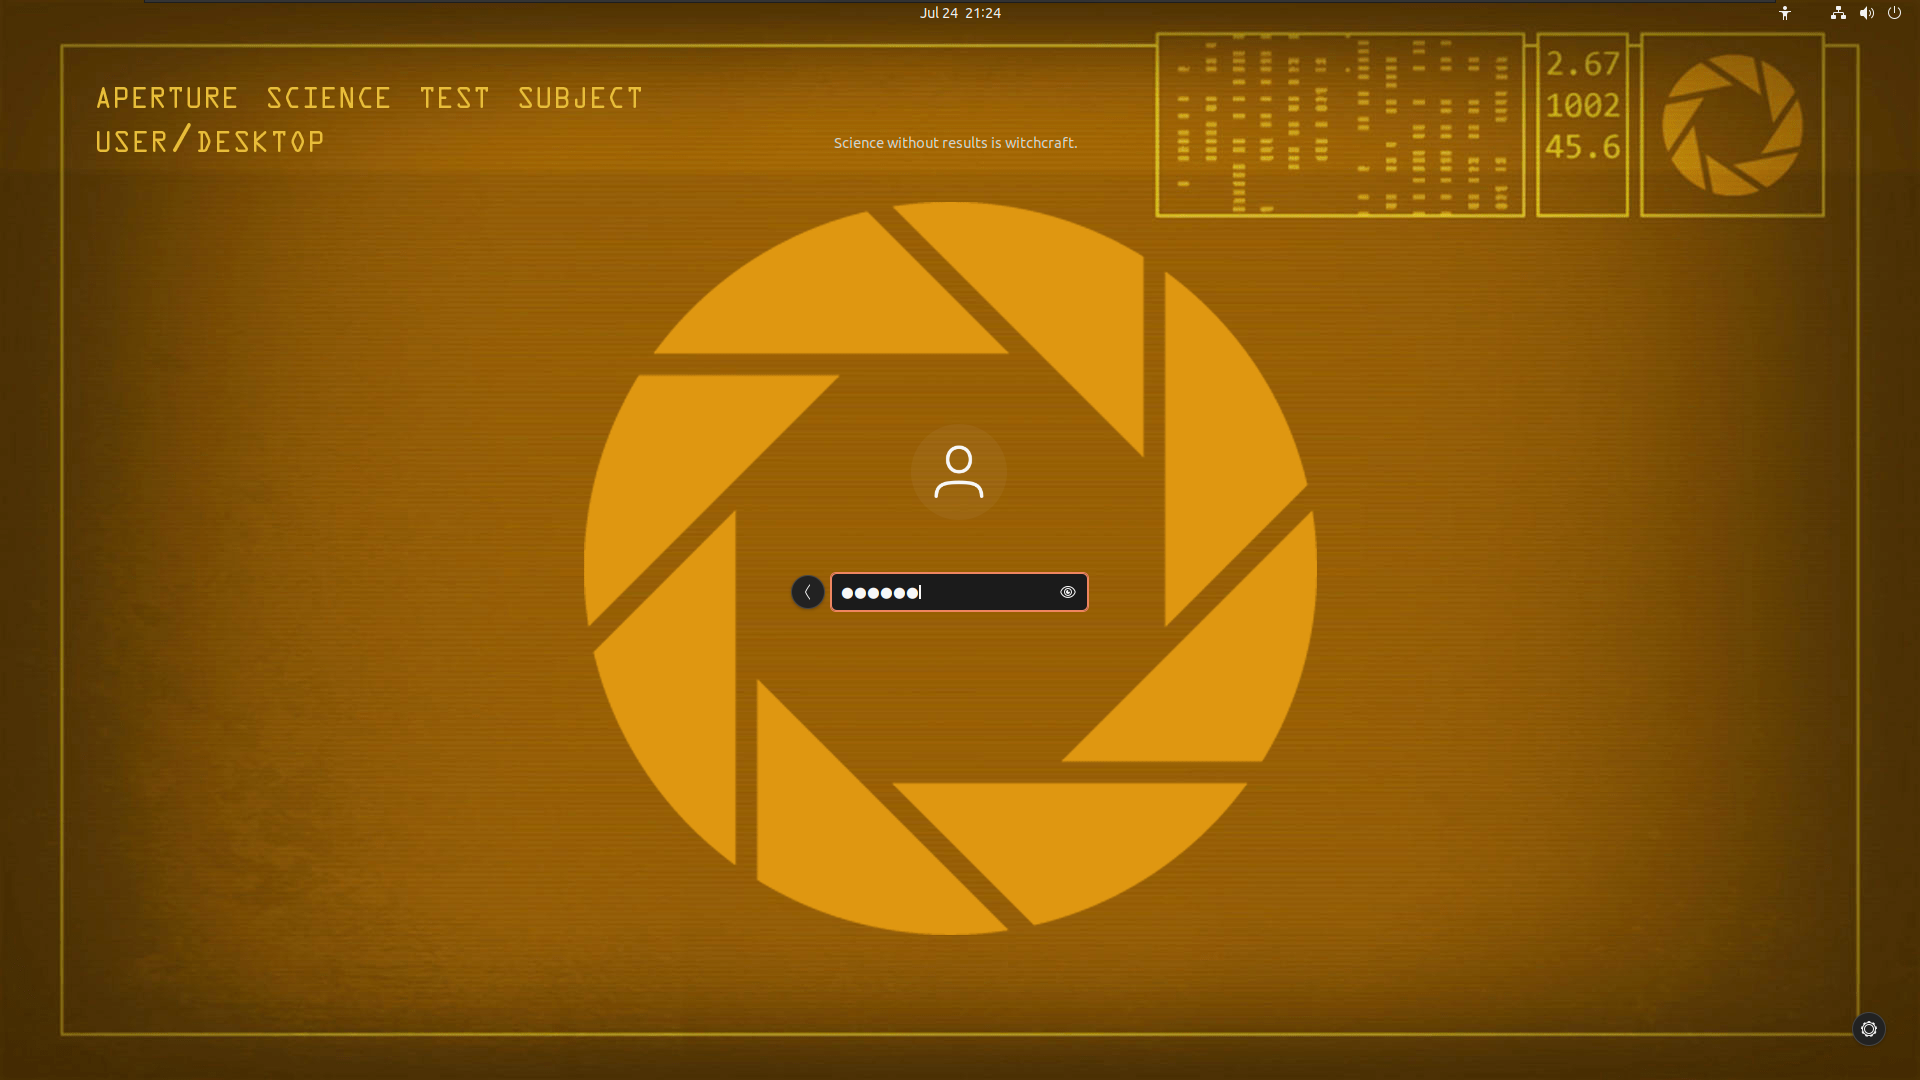
\includegraphics[width=5.20833in,height=\textheight]{img/login-screen.png}

}

\caption{Login screen for the Ubuntu qualifying image}

\end{figure}

\newpage{}

\hypertarget{over-the-wire-09152023}{%
\subsubsection{Over the Wire
(09/15/2023)}\label{over-the-wire-09152023}}

\hypertarget{meeting-summary-2}{%
\paragraph{Meeting Summary}\label{meeting-summary-2}}

In this meeting, students will be divided into teams with 2-4 people per
team, with each team \emph{randomly chosen}. Each team will compete to
see who can reach the highest level on the online wargame
\href{https://overthewire.org/wargames/}{Over The Wire}. This meeting
aims to polish new members' command-line skills and expose them to
essential commands such as \texttt{SSH}, \texttt{find}, \texttt{grep},
and much more. Throughout the entire competition, CyberDragons officers
will be available to help any members that are stuck without giving them
the answers outright. Members may also use the Internet as an
\textbf{educational tool} if they are stuck or have questions, but
directly searching the answers is strictly forbidden. At the end, the
team with the highest level gets free snacks.

\hypertarget{meeting-at-a-glance-2}{%
\paragraph{Meeting At-A-Glance}\label{meeting-at-a-glance-2}}

\begin{itemize}
\tightlist
\item
  Mini CTF (Capture the Flag)-and-terminal-based competition
\item
  Split up into random groups
\item
  Winner incentive (snacks)
\end{itemize}

\hypertarget{cyberdragons-inductions-09222023}{%
\subsubsection{CyberDragons Inductions
(09/22/2023)}\label{cyberdragons-inductions-09222023}}

\hypertarget{meeting-summary-3}{%
\paragraph{Meeting Summary}\label{meeting-summary-3}}

As the official deadline for CyberDragons applications has passed, it is
now time to induct new members into CyberDragons and announce the
CyberPatriot team roster. Additionally, the highest-scoring individual
on the qualifying images will receive a special award. For the rest of
the meeting, CyberPatriot teams will get together and discuss the
qualifying images and upcoming practice round with each other. Returning
members are free to present personal anecdotes about their experiences
in CyberPatriot. To end the meeting, everyone will reconvene to hear
about the logistics of the CyberPatriot official practice round that
will be held the week after.

\hypertarget{meeting-at-a-glance-3}{%
\paragraph{Meeting At-A-Glance}\label{meeting-at-a-glance-3}}

\begin{itemize}
\tightlist
\item
  Celebrate the individual with the most discovered vulnerabilties
\item
  Divide into groups for mostly asynchronous/networking time
\item
  Meet as a collective to discuss logistics for the practice round to
  conclude.
\end{itemize}

\newpage{}

\hypertarget{official-practice-round-10132023}{%
\subsubsection{Official Practice Round
(10/13/2023)}\label{official-practice-round-10132023}}

\hypertarget{meeting-summary-4}{%
\paragraph{Meeting Summary}\label{meeting-summary-4}}

In preparation for our CyberPatriot competitions, members will
collaborate with their teams to complete the official practice round and
practice creating writeups in a Google Doc to familiarize themselves
with the norms of CyberDragons. This meeting will allow members to
experiment with an official CyberPatriot image (developing shell scripts
and README parsers) or work around thier chosen system.

\hypertarget{meeting-at-a-glance-4}{%
\paragraph{Meeting At-A-Glance}\label{meeting-at-a-glance-4}}

\begin{itemize}
\tightlist
\item
  Run through official CyberPatriot images

  \begin{itemize}
  \tightlist
  \item
    The practice round images will be \emph{ten times easier} than the
    qualifying images. Therefore, we expect everyone to ace the images
    and this round should serve as a morale booster.
  \end{itemize}
\item
  Gain experience in working with a team and documenting progress
\end{itemize}

\hypertarget{review-writeups-and-qualifier-images-10202023}{%
\subsubsection{Review Writeups and Qualifier Images
(10/20/2023)}\label{review-writeups-and-qualifier-images-10202023}}

\hypertarget{meeting-summary-5}{%
\paragraph{Meeting Summary}\label{meeting-summary-5}}

With the first official round of CyberPatriot in a day, this meeting
will allow students to reflect on any practice completed during their
time in CyberPatriot. The answer keys for the practice images will be
released during this meeting for members to look at with their teams.
The officers and returning members will be present to assist any burning
questions about the qualifying images and CyberPatriot in general that
newer members may have. It is expected that CyberDragons members review
the forensic questions and vulnerabilities within the qualifying and
practice round images to strengthen their team. It is also \emph{highly
recommended} for CyberDragons members to review writeups for the
practice round and rounds from previous years.

\hypertarget{meeting-at-a-glance-5}{%
\paragraph{Meeting At-A-Glance}\label{meeting-at-a-glance-5}}

\begin{itemize}
\tightlist
\item
  Reflect on completed CyberPatriot practice
\item
  Officers and returning members assist with questions
\item
  Review qualifying images and improve team structure
\item
  Utilize answer keys for the qualifying images
\end{itemize}

\newpage{}

\hypertarget{terminal-teasers-10272023}{%
\subsubsection{Terminal Teasers
(10/27/2023)}\label{terminal-teasers-10272023}}

\hypertarget{meeting-summary-6}{%
\paragraph{Meeting Summary}\label{meeting-summary-6}}

This workshop will begin with a quick introduction to the Bash syntax;
once the introduction ends, every student will be given a reference
sheet to refer to if needed. Students will randomly break into groups of
three and be given a virtual machine with multiple forensic questions.
Each question will be only solvable through a Bash script. Students will
be given a piece of a riddle for every question solved. The first team
to solve all queries and determine the correct answer to the riddle will
be awarded a prize.

\hypertarget{meeting-at-a-glance-6}{%
\paragraph{Meeting At-A-Glance}\label{meeting-at-a-glance-6}}

\begin{itemize}
\tightlist
\item
  Students form groups of three and receive virtual machines with
  forensic questions with a focus on using Bash scripts
\item
  Each solved question provides a riddle piece, and the first team to
  solve the riddle wins a prize
\end{itemize}

\hypertarget{last-meeting-before-round-ii-11032023}{%
\subsubsection{Last Meeting Before Round II
(11/03/2023)}\label{last-meeting-before-round-ii-11032023}}

\hypertarget{meeting-summary-7}{%
\paragraph{Meeting Summary}\label{meeting-summary-7}}

With the second round of CyberPatriot on the following day, this meeting
will be utilized to reflect and review what we did in the first round,
compiling results from both the writeups and reflections written from
the conclusion of the first competition. This meeting will be more
hands-off, prompting more self-reflection and improvements instead of an
informative one.

\hypertarget{meeting-at-a-glance-7}{%
\paragraph{Meeting At-A-Glance}\label{meeting-at-a-glance-7}}

\begin{itemize}
\tightlist
\item
  Members review and reflect what they plan to do differently in the
  second round that they did not do in the first round
\end{itemize}

As a side note, round II of CyberPatriot this year falls on the
\textbf{November SAT} date. So, we'll tell everyone not to sign up for
the November SAT ahead of time.

\newpage{}

\hypertarget{powershell-sherlock-holmes-esque-crime-11102023}{%
\subsubsection{Powershell Sherlock Holmes-esque Crime
(11/10/2023)}\label{powershell-sherlock-holmes-esque-crime-11102023}}

\hypertarget{meeting-summary-8}{%
\paragraph{Meeting Summary}\label{meeting-summary-8}}

The interactive workshop begins with a brief introduction to PowerShell
and its importance in cybersecurity. Following this, students will be
immersed in a crime-solving scenario involving a virtual machine,
enabling them to actively apply PowerShell and develop a deeper
understanding of the tool while sparking their interest. The meeting
aims to familiarize students with PowerShell's practical applications
and promote engagement in the subject.

\hypertarget{meeting-at-a-glance-8}{%
\paragraph{Meeting At-A-Glance}\label{meeting-at-a-glance-8}}

\begin{itemize}
\tightlist
\item
  Introduction to fundamentals of PowerShell:

  \begin{itemize}
  \tightlist
  \item
    Syntax
  \item
    CMDLets
  \item
    PowerShell objects and why everything is an object
  \item
    Pros of Powershell, how it can be used to alter the system
  \end{itemize}
\item
  Reference Materials for people to review and use when working through
  a Powershell interactive challenge
\item
  Model it similar to a Crime Solving Case (centered around Sherlock
  Holmes)
\end{itemize}

\hypertarget{encryptiondecryption-murder-mystery-111723}{%
\subsubsection{Encryption/Decryption Murder Mystery
(11/17/23)}\label{encryptiondecryption-murder-mystery-111723}}

\hypertarget{meeting-summary-9}{%
\paragraph{Meeting Summary}\label{meeting-summary-9}}

In this workshop, participants will receive a concise introduction to
the tools available for decrypting hidden messages. Next, they will
collaborate in randomized teams of 2-4, engaging in a scavenger
hunt-style game that will take them through the main tower of GSMST.
They will decipher clues to uncover the criminal's identity as they
progress through the game. The activity may offer multiple pathways,
allowing students to explore different routes (and not cheat off people
further ahead) and enhance their problem-solving skills.

\hypertarget{meeting-at-a-glance-9}{%
\paragraph{Meeting At-A-Glance}\label{meeting-at-a-glance-9}}

\begin{itemize}
\tightlist
\item
  A murder mystery where students physically walk around the building
\item
  Students use encryption and decryption techniques to decipher clues
  and progress through the game
\end{itemize}

\newpage{}

\hypertarget{computer-forensics-12012023}{%
\subsubsection{Computer Forensics
(12/01/2023)}\label{computer-forensics-12012023}}

\hypertarget{meeting-summary-10}{%
\paragraph{Meeting Summary}\label{meeting-summary-10}}

This meeting will focus on how to approach forensic questions for the
upcoming state round. We will ask new members to share what has worked
for them during previous rounds and then have our veteran members share
their tactics. In addition, we will have our cybersecurity heads will
share their tactics. Once everyone is done sharing, we will review some
practice forensic questions and solve them in groups.

\hypertarget{meeting-at-a-glance-10}{%
\paragraph{Meeting At-A-Glance}\label{meeting-at-a-glance-10}}

\begin{itemize}
\tightlist
\item
  Equip CyberDragons members to solve forensics questions in
  anticipation for the state round
\end{itemize}

\hypertarget{semester-ii}{%
\subsection{Semester II}\label{semester-ii}}

\hypertarget{welcome-back-introduction-to-offensive-security-01122024}{%
\subsubsection{Welcome Back \& Introduction to Offensive Security
(01/12/2024)}\label{welcome-back-introduction-to-offensive-security-01122024}}

\hypertarget{meeting-summary-11}{%
\paragraph{Meeting Summary}\label{meeting-summary-11}}

In this meeting, students will be introduced to the two major
competitions we will focus on this semester: Lockheed Martin CyberQuest
and PicoCTF. With the focus of this semester being CTFs, We will also be
going over a brief explanation of what offensive security is, the
various techniques and types, and how it differs from what students
learned last semester. We will also do a live demo of some CTF problems
after encouraging members to try them first.

\hypertarget{meeting-at-a-glance-11}{%
\paragraph{Meeting At-A-Glance}\label{meeting-at-a-glance-11}}

\begin{itemize}
\tightlist
\item
  Welcome back + here is information on competitions for this semester
\item
  Introduction to offensive security types (Web exploitation, reverse
  engineering, \emph{etc.})
\end{itemize}

\newpage{}

\hypertarget{final-review-before-semifinals}{%
\subsubsection{Final Review Before
Semifinals}\label{final-review-before-semifinals}}

\hypertarget{meeting-summary-12}{%
\paragraph{Meeting Summary}\label{meeting-summary-12}}

This meeting will be celebratory in nature of the various team
accomplishments in CyberPatriot while reviewing and reminding them about
the review materials to assist them for the (probably) final
competition. This meeting may also reflect upon the entire 2023-2024
CyberDragons CyberPatriot experience.

\hypertarget{meeting-at-a-glance-12}{%
\paragraph{Meeting At-A-Glance}\label{meeting-at-a-glance-12}}

\begin{itemize}
\tightlist
\item
  Celebrate CyberDragons' CyberPatriot accomplishments
\item
  Review for the semifinals round
\end{itemize}

\hypertarget{web-exploitation-01192024}{%
\subsubsection{Web Exploitation
(01/19/2024)}\label{web-exploitation-01192024}}

\hypertarget{meeting-summary-13}{%
\paragraph{Meeting Summary}\label{meeting-summary-13}}

This meeting will be going over the basics of Web Hacking, Starting with
OWASP 10 vulnerabilities which consist of commonly found web
applications security vulnerabilities, to techniques such as SQL
injections, Cross Site (XSS) Scripting, and Directory Traversal. In
addition to common techniques, we will also be going over using
BurpSuite, a commonly used tool for web exploitation. We will end this
meeting by having students apply what they learn through interactive
websites like \href{https://www.hackthebox.com/}{HackTheBox} and
\href{https://www.hackthissite.org/}{HackThisSite}.

\hypertarget{meeting-at-a-glance-13}{%
\paragraph{Meeting At-A-Glance}\label{meeting-at-a-glance-13}}

\begin{itemize}
\tightlist
\item
  Introduction to OWASP Top 10 vulnerabilities and common web
  application security issues
\item
  Learn SQL injections, Cross-Site Scripting (XSS), and Directory
  Traversal.
\item
  Familiarization with BurpSuite, a widely used web exploitation tool.
\item
  Apply knowledge on interactive platforms like HackTheBox and
  HackThisSite to gain practical experience.
\end{itemize}

\newpage{}

\hypertarget{command-line-network-penetration-02092024}{%
\subsubsection{Command-line Network Penetration
(02/09/2024)}\label{command-line-network-penetration-02092024}}

\hypertarget{meeting-summary-14}{%
\paragraph{Meeting Summary}\label{meeting-summary-14}}

In this meeting, members will use network tools such as \texttt{netcat}
and \texttt{nmap} to exploit the vulnerabilities of a network or server
through the shell. Additionally, members will learn how to use
\texttt{aircrack-ng} and Wireshark to probe into Wi-Fi networks and
listen and monitor network traffic in real time. First, we will review
basic terminal commands that were touched on in previous meetings, as
well as how to navigate filesystems through the terminal. Then, we will
focus on network penetration through the use of these tools. Finally, we
will focus on practical exercises in hacking servers on HackTheBox.

\hypertarget{meeting-at-a-glance-14}{%
\paragraph{Meeting At-A-Glance}\label{meeting-at-a-glance-14}}

\begin{itemize}
\tightlist
\item
  Recap basic terminal commands and filesystem navigation to prepare for
  network penetration
\item
  Use netcat and nmap to identify and exploit network/server
  vulnerabilities through the shell. Learn to probe and monitor Wi-Fi
  networks using \texttt{aircrack-ng} and Wireshark in real-time.
\end{itemize}

\hypertarget{hacking-tools-02232024}{%
\subsubsection{Hacking Tools
(02/23/2024)}\label{hacking-tools-02232024}}

\hypertarget{meeting-summary-15}{%
\paragraph{Meeting Summary}\label{meeting-summary-15}}

In this workshop, members will learn how to use common hacking tools
such as Metasploit, a versatile penetration testing framework, GDB (GNU
Debugger) for program analysis, SQLMap to uncover web application
vulnerabilities, John The Ripper for advanced password cracking, Hydra
to conduct password attacks, Hashcat for cracking hashed passwords, and
Radare2, an open-source reverse engineering framework for CTF
competitions. Members will be given a problem set where they have to use
these tools, or combinations of them, to solve as many problems as they
can. They can work individually or as a team.

\hypertarget{meeting-at-a-glance-15}{%
\paragraph{Meeting At-A-Glance}\label{meeting-at-a-glance-15}}

\begin{itemize}
\tightlist
\item
  Learn how to use various hacking tools like Metasploit, GDB, SQLMap,
  John The Ripper, Hydra, Hashcat, and Radare2.
\item
  Members will receive a problem set and use the tools to solve
  vulnerabilities and challenges
\item
  Gain hands-on experience with tools used in penetration testing,
  password cracking, web app vulnerability discovery, and reverse
  engineering
\item
  Engage in problem-solving similar to CTF competitions to apply
  acquired skills effectively
\end{itemize}

\hypertarget{steganographic-art-gallery-03012024}{%
\subsubsection{Steganographic Art Gallery
(03/01/2024)}\label{steganographic-art-gallery-03012024}}

\hypertarget{meeting-summary-16}{%
\paragraph{Meeting Summary}\label{meeting-summary-16}}

Students will be introduced to steganography as an art of concealing
information through digital media files and byte/color channel
manipulation. We will expose our members to various steganography
techniques and have them create their own hidden messages through
(school appropriate) images. Towards the end of the meeting, we will
have a steganography ``art gallery,'' where members rotate to a new
device clockwise every minute to take a look at that at that laptop's
steganographic images and the creator's instructions on how to decode
them. And then they attempt to decode the images for each computer,
hopefully successfully most of the time!

\hypertarget{meeting-at-a-glance-16}{%
\paragraph{Meeting At-A-Glance}\label{meeting-at-a-glance-16}}

\begin{itemize}
\tightlist
\item
  Explore the art of concealing information within digital media files
  using steganography techniques.
\item
  Members will create their own hidden messages within
  school-appropriate images with instructions on how to decode them
\item
  Rotate through laptops, viewing and successfully decoding
  steganographic images created by fellow members
\item
  Foster an enjoyable environment for learning steganography through
  practical application and peer interaction
\end{itemize}

\begin{figure}

{\centering 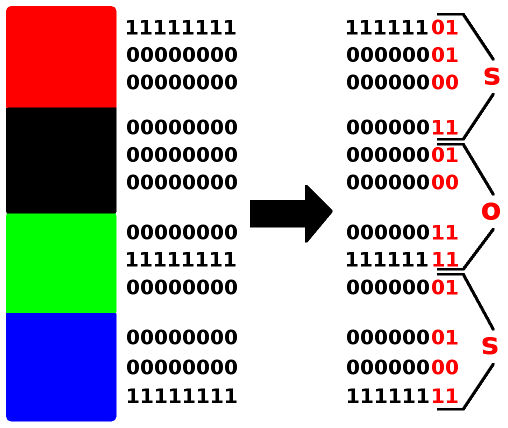
\includegraphics[width=3.64583in,height=\textheight]{img/LSB_example.jpg}

}

\caption{An example of Least Significant Bit steganography}

\end{figure}

\hypertarget{review-session-for-lockheed-martin-cyberquest-and-picoctf-03082024}{%
\subsubsection{Review Session for Lockheed Martin CyberQuest and picoCTF
(03/08/2024)}\label{review-session-for-lockheed-martin-cyberquest-and-picoctf-03082024}}

\hypertarget{meeting-summary-17}{%
\paragraph{Meeting Summary}\label{meeting-summary-17}}

This meeting will consist of a review of the last four meetings in
preparation for next week's picoCTF competition. Once review is over,
students will be given a Kahoot to test their knowledge and highlight
any parts they lack. For the excess time, students will break themselves
into groups and work on some practice problems on picoGym to prepare for
actual CTF questions.

\hypertarget{meeting-at-a-glance-17}{%
\paragraph{Meeting At-A-Glance}\label{meeting-at-a-glance-17}}

\begin{itemize}
\tightlist
\item
  Engage members with a Kahoot to test their knowledge and identify
  areas that need improvement
\item
  Utilize excess time for hands-on learning on
\end{itemize}

\hypertarget{picoctf-competition-meeting-03222024}{%
\subsubsection{picoCTF Competition Meeting
(03/22/2024)}\label{picoctf-competition-meeting-03222024}}

\hypertarget{meeting-summary-18}{%
\paragraph{Meeting Summary}\label{meeting-summary-18}}

Students work on US Cyber Challenge: Cyber Quests or picoCTF
asynchronously with their teams.

\hypertarget{meeting-at-a-glance-18}{%
\paragraph{Meeting At-A-Glance}\label{meeting-at-a-glance-18}}

\begin{itemize}
\tightlist
\item
  Work on picoCTF or Cyber Quests
\end{itemize}

\newpage{}

\hypertarget{picoctf-award-ceremony-03292024}{%
\subsubsection{picoCTF Award Ceremony
(03/29/2024)}\label{picoctf-award-ceremony-03292024}}

\hypertarget{meeting-summary-19}{%
\paragraph{Meeting Summary}\label{meeting-summary-19}}

This meeting will start with an award ceremony honoring our top three
highest achieving teams (If there are less than six teams, we will
reduce the ceremony to award to the top team only). After the award
ceremony, there will be a group discussion about any pitfalls and traps
that participating teams encountered and any helpful strategies that
helped them succeed in this year's competition. Once the group
discussion is over, the heads will review any CTF questions members
have.

\hypertarget{meeting-at-a-glance-19}{%
\paragraph{Meeting At-A-Glance}\label{meeting-at-a-glance-19}}

\begin{itemize}
\tightlist
\item
  Award top-performing team(s) in picoCTF
\item
  Review strategies and pitfalls
\item
  Go over questions
\end{itemize}

\hypertarget{chill-04192024}{%
\subsubsection{Chill (04/19/2024)}\label{chill-04192024}}

\hypertarget{meeting-summary-20}{%
\paragraph{Meeting Summary}\label{meeting-summary-20}}

We are planning to organize an end-of-year party to celebrate our
accomplishments during this school year. We will also discuss our future
goals and aspirations for the upcoming years. Lastly, we will bid
farewell to our senior club members and spend the remaining time
unwinding.

\hypertarget{meeting-at-a-glance-20}{%
\paragraph{Meeting At-A-Glance}\label{meeting-at-a-glance-20}}

\begin{itemize}
\tightlist
\item
  Celebrate accomplishments
\item
  Talk about the future of CyberDragons
\item
  Relax
\end{itemize}



\end{document}
